La siguiente pirámide cuadrangular tiene altura inclinada de 17 unidades y
su altura vertical es 15 unidades, como se muestra en la figura \ref{fig:pitagoras3D_piram_01}:\\
\begin{figure}[H]
    \begin{center}
        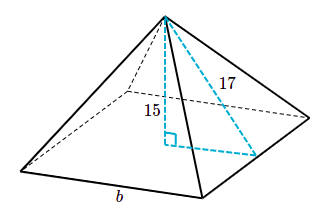
\includegraphics[width=0.4\textwidth]{../images/pitagoras3D_piram_01.png}
    \end{center}
    \caption{}
    \label{fig:pitagoras3D_piram_01}
\end{figure}
\textbf{¿Cuál es la longitud $b$ de un lado de la base de la pirámide?}\\